%%%%%%%%%%%%%%%%%%%%%%%%%%%%%%%%%%%%%%%%%%%%%%%%%%%%%%%
%%%%%%%%%%%%%%%%%%%%%%%%%%%%%%%%%%%%%%%%%%%%%%%%%%%%%%%
%%%%%%%%%%%%%%%%%%%%%%%%%%%%%%%%%%%%%%%%%%%%%%%%%%%%%%%
% PREAMBLE:

\documentclass[12pt,a2paper,landscape]{article}

%%%%%%%%%%%%%%%%%%%%%%%%%%%%%%%%%%%%%%%%%%%%%%%%%%%%%%%

\usepackage[noheadfoot,margin=10mm]{geometry}
% width=554mm,height=400mm
\usepackage[utf8]{inputenc}
\usepackage[english]{babel}
\usepackage{graphicx,multicol,color} 
%\usepackage{everyshi,eso-pic,calc,ifthen,wallpaper} 
\usepackage{tikz}
\usepackage{amsmath,amsfonts,amssymb,amsthm}
\usetikzlibrary{automata,arrows,positioning,calc}
\usepackage{mathtools}
\usepackage{caption}
\usepackage{anyfontsize}

%%%%%%%%%%%%%%%%%%%%%%%%%%%%%%%%%%%%%%%%%%%%%%%%%%%%%%%

\pagestyle{empty}
\definecolor{cola}{rgb}{.99,.93,0}
\definecolor{colb}{rgb}{.8,0,.7}
\definecolor{colc}{rgb}{1,.9,.9}
\DeclarePairedDelimiter\abs{\lvert}{\rvert}

%% boxes to put stuff in ......
%%
%%   (1) transparent boxes --- the background shows through
%%			   #1 = width as fraction of what's available
%%                         #2 = contents (text, formula, picture)
%%                               ... tho pictures are always opaque
%% ---- box for headers --- width = fraction of textwidth 

\newcommand\BoX[2]{\begin{minipage}{#1\textwidth}#2\end{minipage}}
%% ---- box centred in a column --- width = fraction of columnwidth
\newcommand\BOX[2]{\begin{center}
   \begin{minipage}{#1\columnwidth}#2\end{minipage}\end{center}\vfill}
%%
%%   (2) opaque boxes with coloured background and outline frame
%%                         #1 = width as fraction of what's available
%%                         #2 = contents (text, formula, picture)
%%                         #3 = background colour
%%                         #4 = frame colour
\setlength\fboxrule{2pt} %% = width of frame lines round boxes
\setlength\fboxsep{5pt}  %% = spacing round box contents
%% ---- box for headers --- width = fraction of textwidth 
\newcommand\cBoX[4]{\fcolorbox{#4}{#3}{%
	\begin{minipage}{#1\textwidth}#2\end{minipage}}}
%% ---- box centred in a column --- width = fraction of columnwidth
\newcommand\cBOX[4]{\begin{center}\fcolorbox{#4}{#3}{%
 \begin{minipage}{#1\columnwidth}#2\end{minipage}}\end{center}\vfill}


%% for e.g. picture and text side-by-side in a column
%%   n.b. this command must be inside a \BOX or a \cBOX
\newcommand\sidebyside[2]{\BoX{.485}{#1}\BoX{.485}{#2}}

\def\bibsection{\section*{References}}        % Position reference section correctly

\renewcommand\familydefault{\sfdefault}

\newtheorem{definition}{Definition}[section]
\newtheorem{exmp}{Example}[section]
\newtheorem*{theorem*}{Theorem}
\DeclareMathOperator{\sech}{sech}		% Defining sech so it doesn't italicise it 
\DeclareMathOperator{\Int}{Int}		% Defining 'integer part of' so it doesn't italicise it 

\setlength\columnsep{10mm}  %%%% column separation

%%%%%%%%%%%%%%%%%%%%%%%%%%%%%%%%%%%%%%%%%%%%%%%%%%%%%%%
%%%%%%%%%%%%%%%%%%%%%%%%%%%%%%%%%%%%%%%%%%%%%%%%%%%%%%%
%%%%%%%%%%%%%%%%%%%%%%%%%%%%%%%%%%%%%%%%%%%%%%%%%%%%%%%
% DOCUMENT

\begin{document}
%\tikz[remember picture,overlay] \node[inner sep=0pt] at (current page.center)
%{ 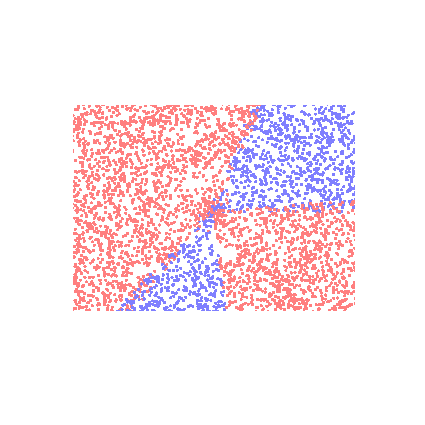
\includegraphics[width=\paperwidth,height=\paperheight]{spiral3.pdf}};

\begin{tikzpicture}[remember picture, overlay]
  \node [anchor=north west, inner sep=1cm]  at (current page.north west)
     {
\includegraphics[height=3cm]{university1}};
\end{tikzpicture}
\hfill
\cBoX{0.75}{\centering
\vspace{1ex}
{\fontsize{1.8cm}{2cm}\selectfont{\textsc{Collisions of Matter-Wave Solitons \\}}}
\huge
\textsc{Lois P Flower\\ %L P Flower? 
Project Tutor: Dr. Rahul Sawant}
\vspace{1ex}
}{white}{white}
\hfill
%\cBoX{.3}{\color{black}
%\centering
%\huge
%\textsc{L P Flower\\
%Project Tutor: \\
%Dr. Rahul Sawant}
%}{white}{white}
\vspace{0.5in} 

%%%%%%%%%%%%%%%%%%%%%%%%%%%%%%%%%%%%%%%%%%%%%%%%%%%%%%%
%%%%%%%%%%%%%%%%%%%%%%%%%%%%%%%%%%%%%%%%%%%%%%%%%%%%%%%
%%%  now the body material in 3 columns of stacked boxes
%%      ... use \BOX and/or \cBOX here

\begin{multicols*}{3}
\setlength\fboxrule{1pt} 

%%%   to get more in, try say 4 columns with smaller-sized type
%%%  BUT -- for easy reading 
%%%               use no more than about 66 characters per line
%%%%   .... and choose a size of type that 
%%%%              looks OK expanded from A4 to A2
% \tiny
\small


%%%%%%%%%%%%%%%%%%%%%%%%%%%%%%%%%%%%%%%%%%%%%%%%%%%%%%%

\fboxsep=5.5pt

\cBOX{0.97}{\section*{{\fontsize{28pt}{35pt}\selectfont Introduction}}
{
\fontsize{16pt}{20pt}\selectfont
The atoms in a Bose-Einstein condensate are all described by the same wavefunction, since they are in the same quantum state, which includes each atom's interaction with the other atoms in the condensate. Introducing an pseudopotential term $g \abs{\psi}^2$ which characterises the interactions between the particles into the dimensionless Schr\"{o}dinger equation yields the Gross-Pitaevskii equation \cite{Gross}\cite{Pitaevskii}
\begin{equation}
i \frac{\partial \psi}{\partial t} = -\frac{\partial^2 \psi}{\partial x^2} + (V + g \abs{\psi}^2) \psi,
\end{equation}
where $\psi$ is the atomic wavefunction, $t$ and $x$ are the rescaled time and length variables, $V$ is the external potential (if present) and $g$ is the interaction parameter. 

It is usual to define $\zeta$ as a parameter to characterise width, with units of inverse length. The normalised wavefunction is then
\begin{equation} 
\psi(x) = \sqrt{\frac{\zeta}{2}} \sech{(\zeta x)} e^{i v x + \phi},
\end{equation}
where $v$ is the velocity of the soliton and $\phi$ is a phase factor. 
Substituting the $v=0$ case into the time-independent Schrodinger equation and setting E to be $\zeta^2$ to eliminate $x$, we find $g=-4\zeta$.

\vspace{1ex}
\section*{{\fontsize{28pt}{35pt}\selectfont Propagating a Soliton}}

The Gross-Pitaevskii equation was solved numerically using the split-step Fourier method for rescaled time $t$. The space-time box was initially 20x20, and was increased to 40x40 for repeated collisions. 4000 space points and 4000 time points were used to minimise discretization effects. For $\zeta=1$, it was found by trial and error that $g=-4$ confined the soliton, in perfect agreement with theory. 

\begin{center}
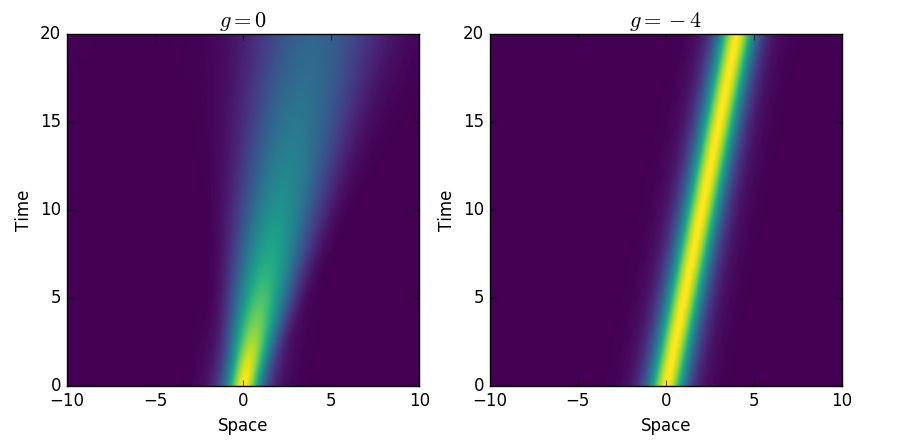
\includegraphics[width=\columnwidth]{milestonepic.png}
\captionof{figure}{A graph showing the effect of inter-atom interactions $g \abs{\psi^2}$ on a soliton model. The family 
parameter $\zeta = 1$ hence $g=-4$ perfectly confines the soliton with velocity $v=0.2$.}
\end{center}
}
}{white}{white}

%%%%%%%%%%%%%%%%%%%%%%%%%%%%%%%%%%%%%%%%%%%%%%%%%%%%%%%

\columnbreak
\cBOX{0.97}{\section*{{\fontsize{28pt}{35pt}\selectfont Soliton Collisions}}
{
\fontsize{16pt}{20pt}\selectfont

Two solitons were created at positions symmetrical about zero and given equal and opposite velocities to cause them to collide roughly halfway through the time period modelled. The resulting dynamics were plotted for different values of the interaction parameter $g$, two of which are plotted below (see Fig.2). For small negative values of $g$, the solitons are fairly diffuse initially and produce a large interference pattern when they collide, but emerge with their velocities and relative phase unchanged. Large negative $g$ values and hence very narrow solitons have intuitively stranger collision properties, seeming to 'bounce off' one another when in antiphase. This is due to the wave properties of the condensate and is not indicative of the constituent atoms actually undergoing elastic collisions. For relative phases of $\pi/2$ and $3\pi/2$, not shown here, the interference pattern is asymmetrical.

\begin{center}
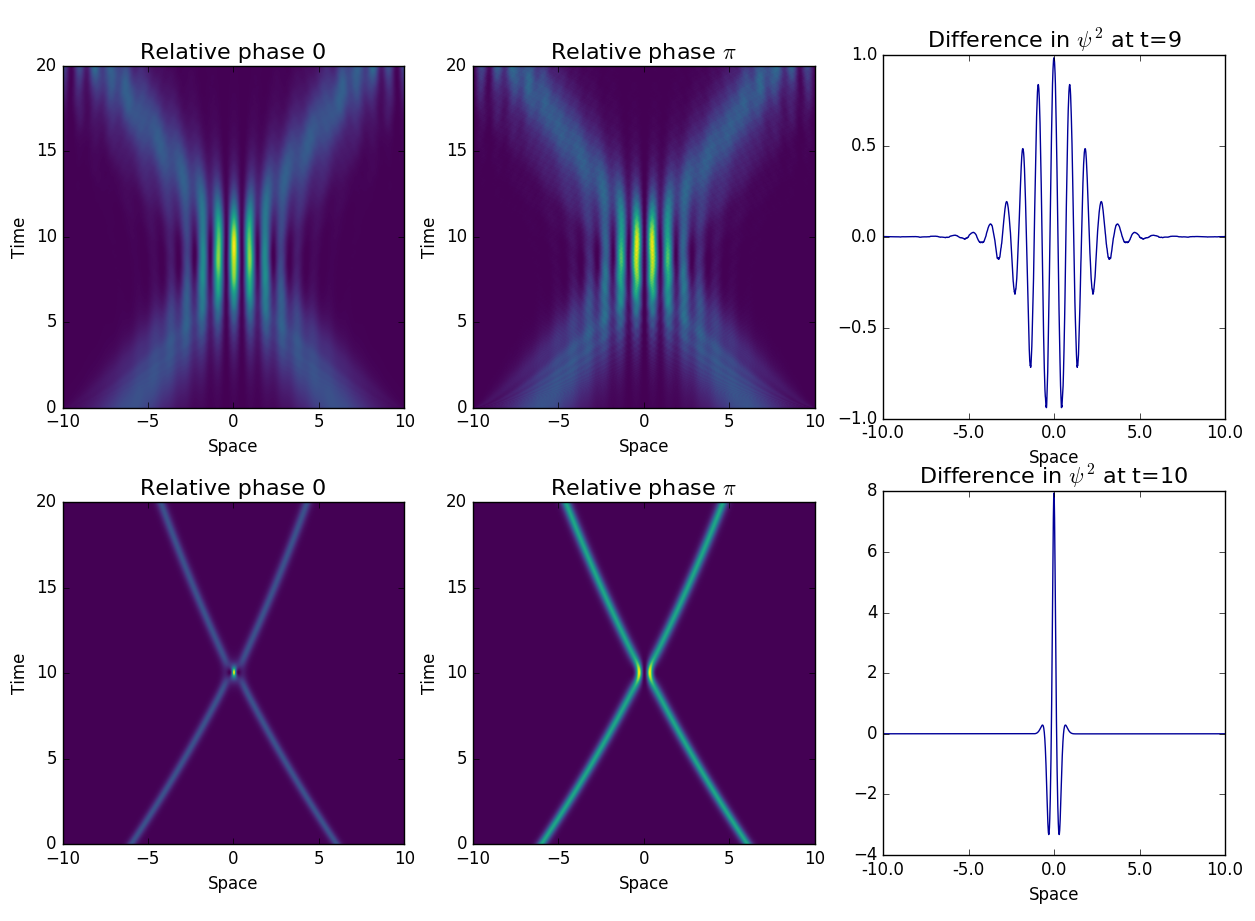
\includegraphics[width=\columnwidth]{extensionpic.png}
\captionof{figure}{Two colliding solitons, in phase and in antiphase. The top row have $g=-2$ corresponding to $\zeta=0.5$ whilst the bottom row have $g=-12$, $\zeta=4$. Both sets of solitons have velocities $\abs{v}=2/3$.}
\end{center}

At first glance, the two phase cases for $g=-2$ (see Fig.2 top row) look very similar. In reality, where the solitons are in phase at the time of collision there is a central bright fringe in the interference pattern, as opposed to a central dark fringe in the antiphase case. The rightmost plot is included to illustrate this, showing the difference $\psi_0^2 - \psi_{\pi}^2$ at the time of collision. 

When narrow solitons collide (see Fig.2 bottom row), the resulting interference resembles a particle-particle interaction, especially in the antiphase case. However, the strong interactions seem to have caused an attractive force between the solitons as evidenced by the final separation of $\Delta x = 9$ compared to the initial separation of $\Delta x=12$. This result is somewhat unexpected as solitons should not affect each other even under collisions. It is possible that the solitons were not well-separated so formed a short-lived 'bound state' \cite{Bound}.

}
}{white}{white}

%%%%%%%%%%%%%%%%%%%%%%%%%%%%%%%%%%%%%%%%%%%%%%%%%%%%%%%

\columnbreak
\cBOX{0.97}{\section*{{\fontsize{28pt}{35pt}\selectfont Repeated Collisions}}

{\fontsize{16pt}{20pt}\selectfont
Introducing a weak harmonic potential to the 1D Bose-Einstein condensate model confines the solitons axially within the box. After a collision the solitons climb a distance up the potential barrier dictated by their momentum (and hence velocity) and return to collide again. The axial potential preserves the relative phase and velocity of the solitons, allowing perfect periodic motion. However, the introduction of this potential places limits on the range of interaction parameters $g$ which lead to soliton-like behaviour.

\vspace{1ex}
\begin{center}
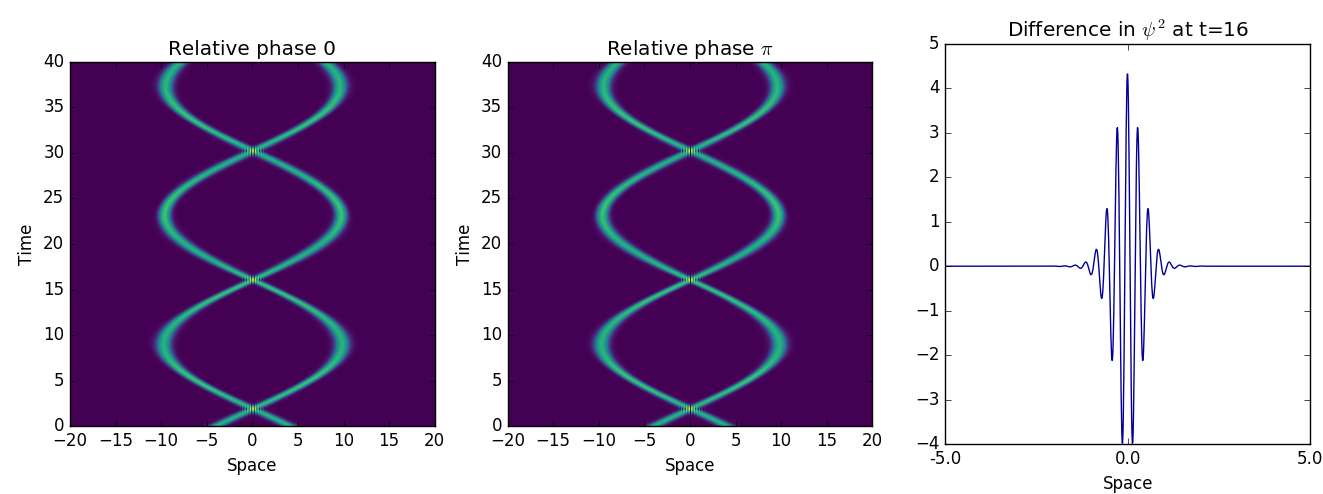
\includegraphics[width=\columnwidth]{difference-g7.png}
\captionof{figure}{Two solitons with starting positions $-4$ and $4$ and velocities $2$ and $-2$, with relative phase either $0$ or $\pi$ radians. The interaction parameter $g=-7$ thus $\zeta=1.75$. The images here are plotted on a symmetric log scale with a linear cutoff of $\psi^2 = 0.3$ to improve visibility of the solitons.}
\end{center}

It was observed that for $g \leq 4$, the solitons were affected adversely by the external potential and appeared diffuse. For $g \geq 12$ a numerical limit of the model was reached and the solitons lost energy in subsequent collisions. The model is valid for interaction parameters between these values, corresponding to family parameters $1 < \zeta < 3$.

It is possible to model matter-wave solitons as classical particles due to the phase-independence of the solitons' behaviour after a collision \cite{Adams}. Qualitatively, the regimes explored in this part of the experiment seem to be suitable for modelling as classical particles. 
}
}{white}{white}

%%%%%%%%%%%%%%%%%%%%%%%%%%%%%%%%%%%%%%%%%%%%%%%%%%%%%%%

\vspace{-2cm}
\cBOX{0.97}{\section*{{\fontsize{24pt}{30pt}\selectfont Final Remarks}}
{\fontsize{16pt}{20pt}\selectfont
To investigate whether the extent and parameters used here are well explained by a particle model, an effective inter-soliton potential will be introduced and the dynamics of the 'particles' observed. 

It would also be interesting to introduce a third soliton and observe subsequent chaotic dynamics in certain regimes, analogous to the classical three-body problem. 
}
}{white}{white}

%%%%%%%%%%%%%%%%%%%%%%%%%%%%%%%%%%%%%%%%%%%%%%%%%%%%%%%

\vspace{-2cm}
\cBOX{0.97}{

\begin{thebibliography}{}

\bibitem{Gross} E. P. Gross (1961), "Structure of a quantised vortex in boson systems", \textit{Il Nuovo Cimento}, \textbf{20}(3) pp. 454-477. 
\bibitem{Pitaevskii}  L. P. Pitaevskii (1961), "Vortex lines in an imperfect Bose gas", \textit{Sov. Phys. JETP.} \textbf{13}(2) pp. 451–454.
\bibitem{Bound} N.-C. Panoiu, I. V. Mel’nikov, D. Mihalache, C. Etrich and F. Lederer (1999), "Multiwavelength pulse transmission in an optical fibre - Amplifier system", \textit{Phys. Rev.} \textbf{60}(4868).
\bibitem{Adams} A. D. Martin, C. S. Adams and S. A. Gardiner (2008), "Bright Solitary-Matter-Wave Collisions in a Harmonic Trap: Regimes of Soliton-like Behaviour", \textit{Physical Review A} \textbf{77}(1). 

\end{thebibliography} 

}{white}{white}
\end{multicols*}
\end{document}

%%%%%%%%%%%%%%%%%%%%%%%%%%%%%%%%%%%%%%%%%%%%%%%%%%%%%%%
%%%%%%%%%%%%%%%%%%%%%%%%%%%%%%%%%%%%%%%%%%%%%%%%%%%%%%%